% Created 2015-11-27 Fri 18:40
\documentclass{article}
\usepackage[top=1in, bottom=1.in, left=1in, right=1in]{geometry}
  \usepackage[makeroom]{cancel}
\usepackage{verbatim}


\usepackage[utf8]{inputenc}
\usepackage{lmodern}
\usepackage[T1]{fontenc}
\usepackage{fixltx2e}
\usepackage{graphicx}
\usepackage{longtable}
\usepackage{float}
\usepackage{wrapfig}
\usepackage{rotating}
\usepackage[normalem]{ulem}
\usepackage{amsmath}
\usepackage{textcomp}
\usepackage{marvosym}
\usepackage{wasysym}
\usepackage{amssymb}
\usepackage{amsmath}
\usepackage[version=3]{mhchem}
\usepackage[numbers,super,sort&compress]{natbib}
\usepackage{natmove}
\usepackage{url}
\usepackage{minted}
\usepackage{underscore}
\usepackage[linktocpage,pdfstartview=FitH,colorlinks,
linkcolor=blue,anchorcolor=blue,
citecolor=blue,filecolor=blue,menucolor=blue,urlcolor=blue]{hyperref}
\usepackage{attachfile}
\author{Abhishek Bagusetty}
\date{\today}
\title{24-623 2015 HM6}
\begin{document}

\maketitle

\section{Problem 1}
\label{sec-1}
\subsection{Computational configuration}
\label{sec-1-1}
\begin{enumerate}
\item An atom is randomly selected and moved per trial move and it is important to note that the atom randomly selected is distinct from the last move.
\item Equlibration is completed, as judged by the lack of drift to potential energy in the 200000 movies of MC simulation. $\big\langle (U -\langle U \rangle) \big\rangle$ per atom is in the order of 1e-3 which indicate the energy fluctuations are very small and the system is equilibrated.
\item To find appropriate max. step size required for the Metropolis MC simualtion, various runs with step sizes of 0.05, 0.01, 0.5 is performed and the potential energy variation is compared with the MD-NVT simulation.
\end{enumerate}

\subsection{a)}
\label{sec-1-2}
\begin{figure}[htb]
\centering
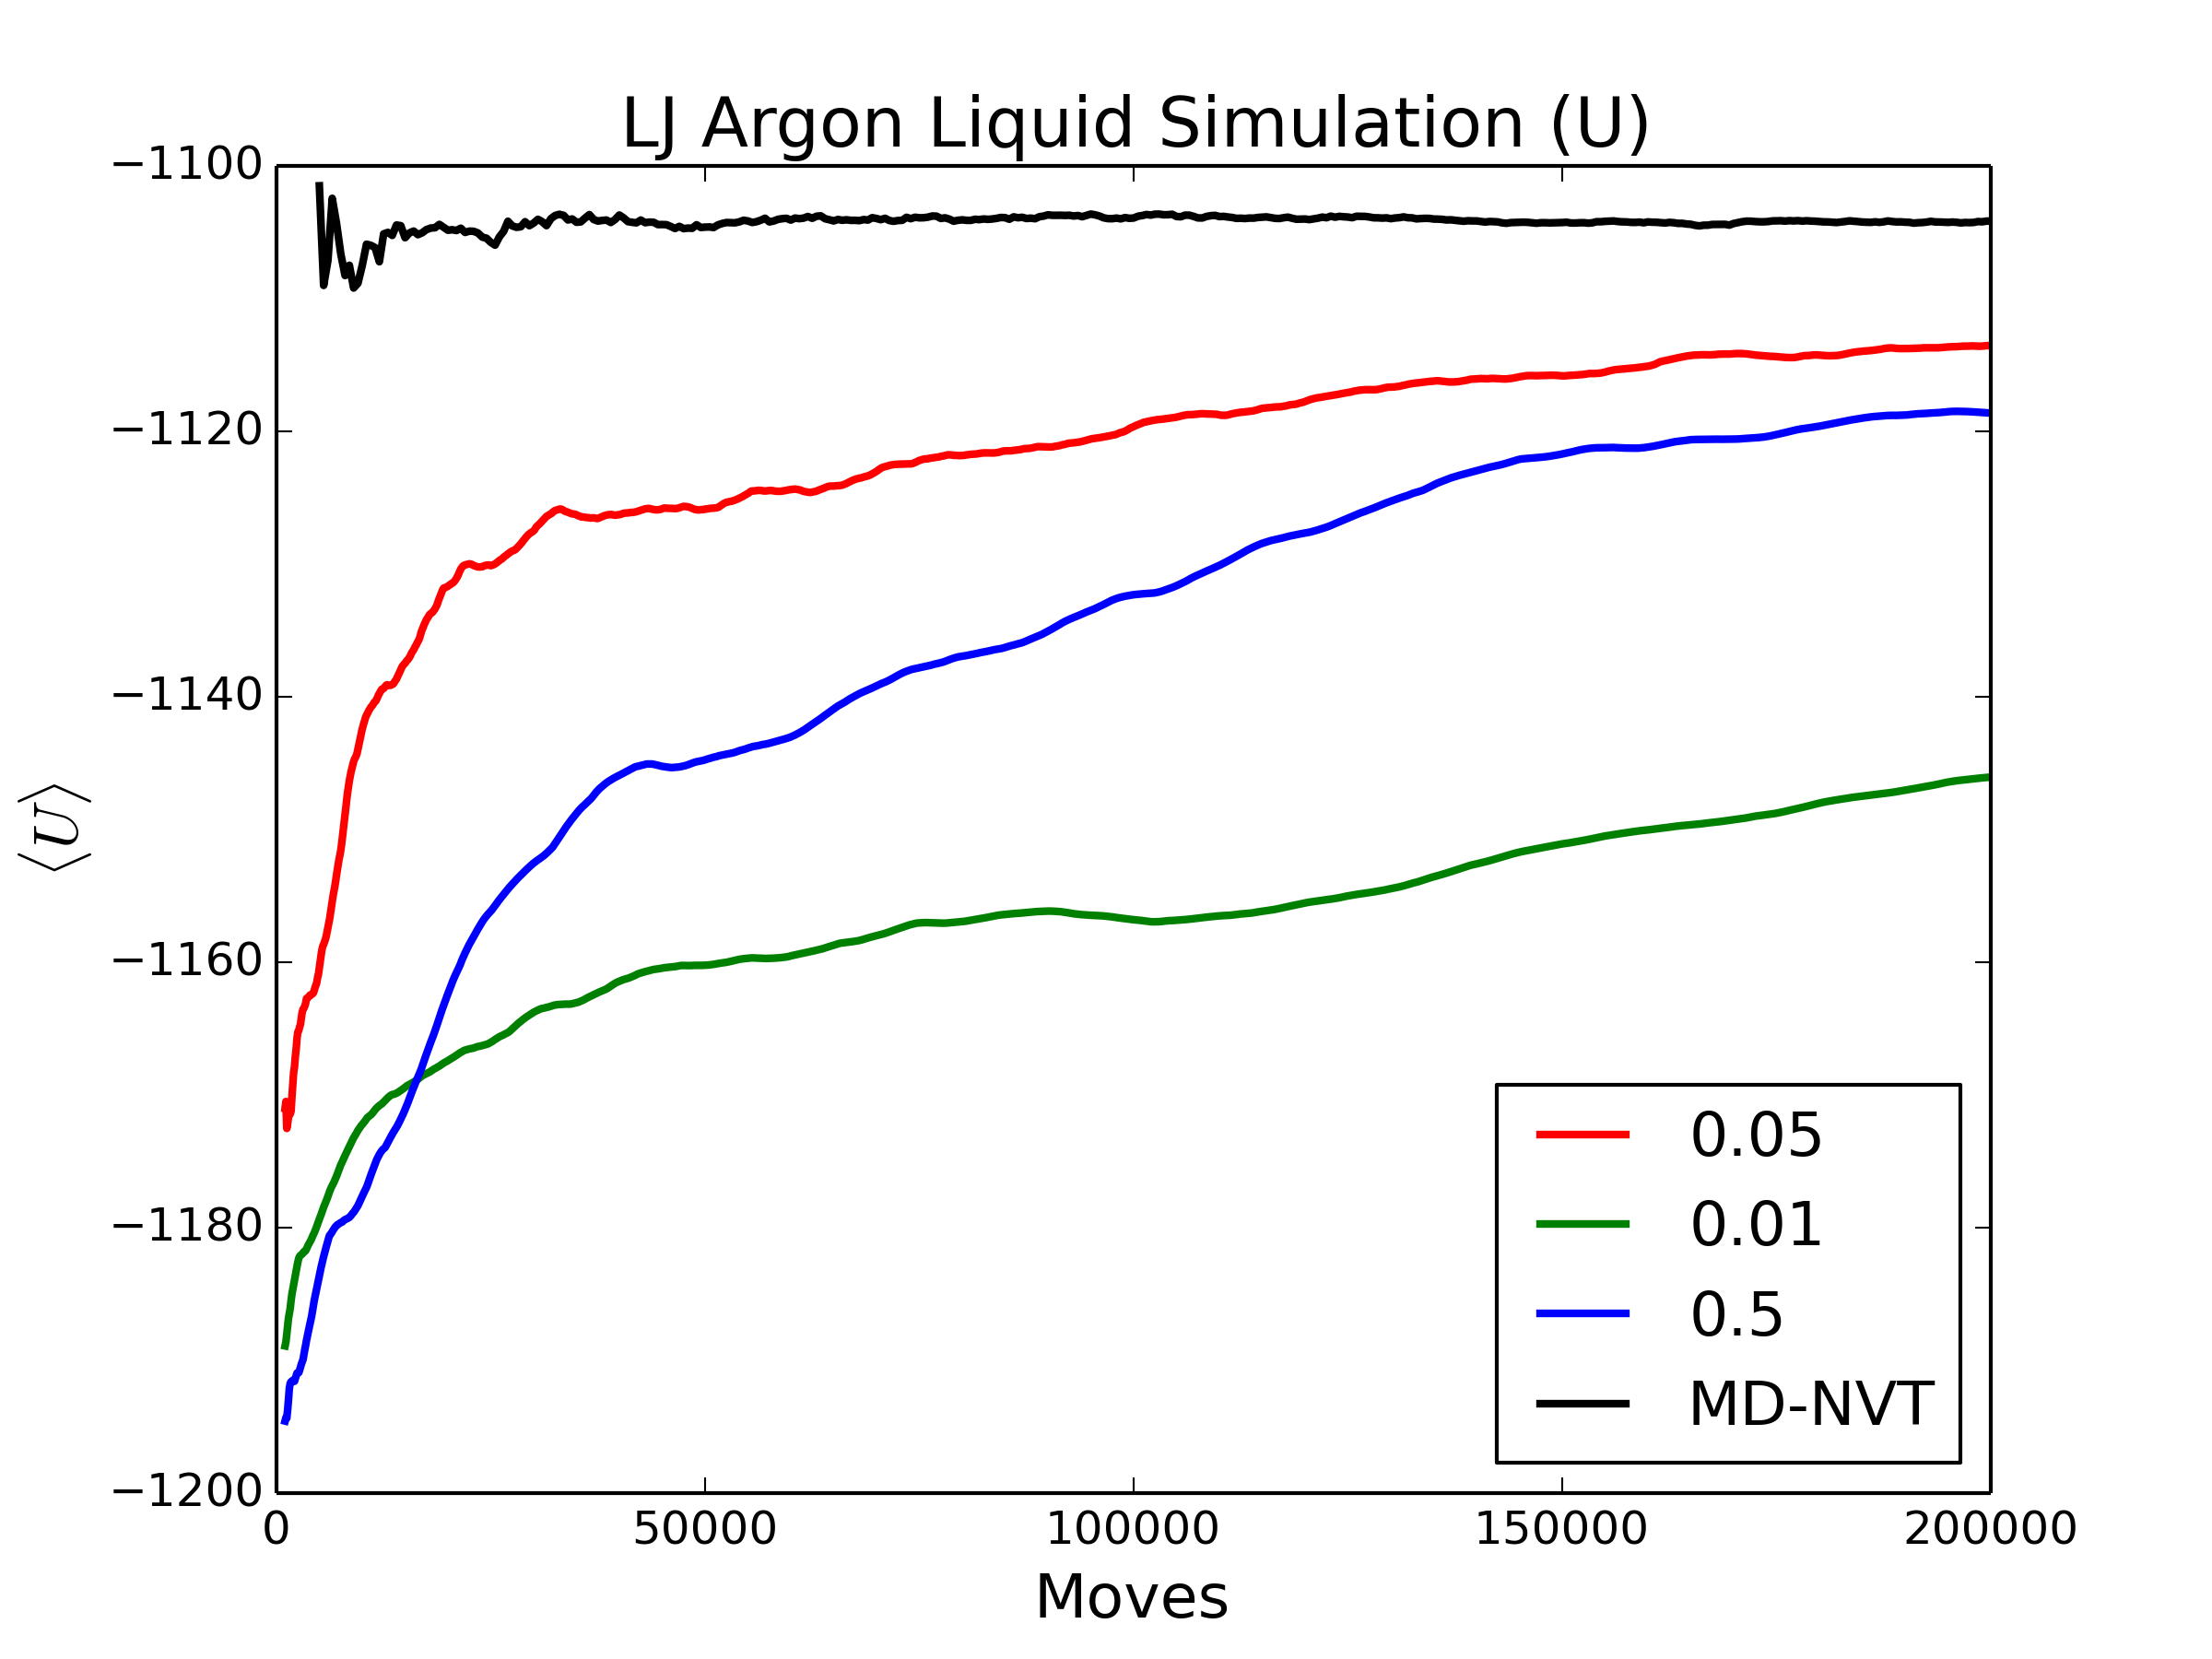
\includegraphics[width=.9\linewidth]{./P1/LJ-md-Ener.png}
\caption{\label{fig:P1a-energy}The figure shows the relation evolution of $\langle U \rangle$ with trial moves at the different max. step sizes of 0.05, 0.01, 0.5 along with the value for MD-NVT simulation.}
\end{figure}

It is very evident from the above Fig.\ref{fig:P1a-energy} that the ideal step size of 0.05 is valid for MC simulation depending upon the fluctuations and convergence when compared to the MD-NVT simuation carried out at the same conditions.

\begin{figure}[htb]
\centering
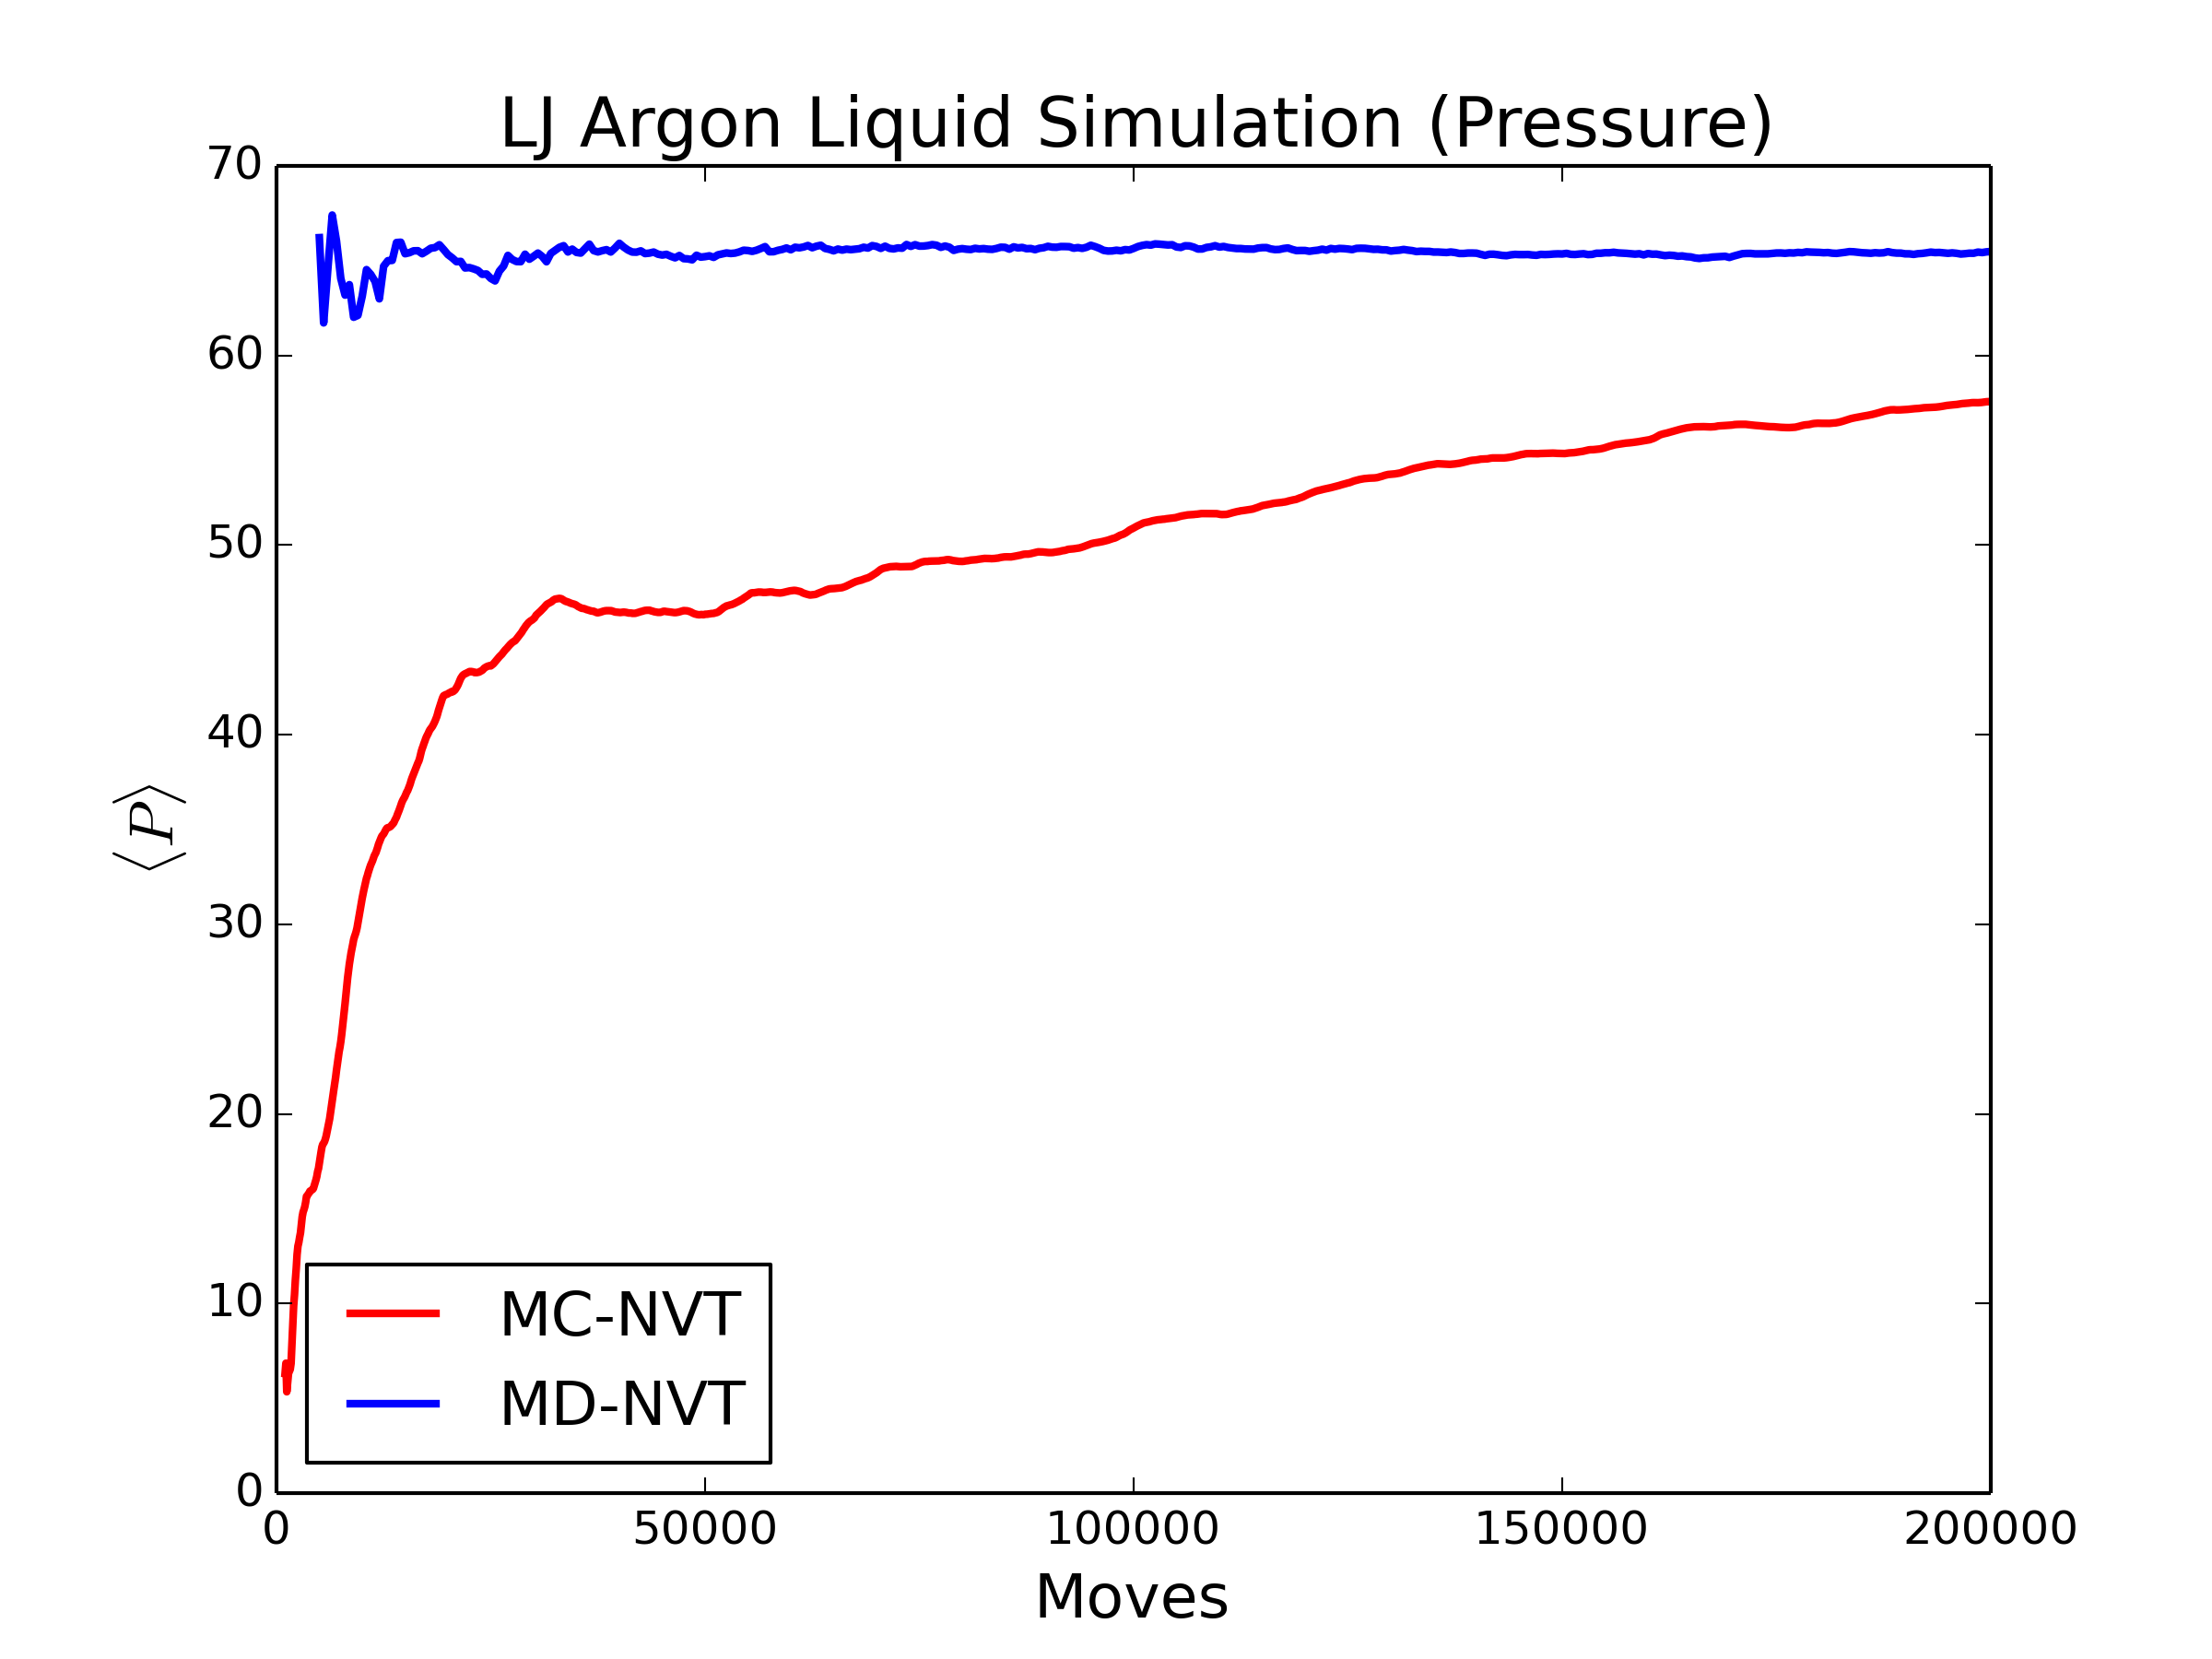
\includegraphics[width=.9\linewidth]{./P1/LJ-md-Pressure.png}
\caption{\label{fig:P1b-pressure}The figure shows the relation evolution of $\langle P \rangle$ with trial moves at the max. step size of 0.05}
\end{figure}

The value of $\langle U \rangle$ using metropolis montecarlo simulation is obtained to be -1113.542 , when compared to the value of -1104.155 obtained from MD-NVT simulation. On the same lines, $\langle P \rangle$ of 58.5700 MPa is obtained from MC NVT simulation when compared to 65.50 MPa obtained from MD NVT simulation.

\subsection{b)}
\label{sec-1-3}
\begin{figure}[htb]
\centering
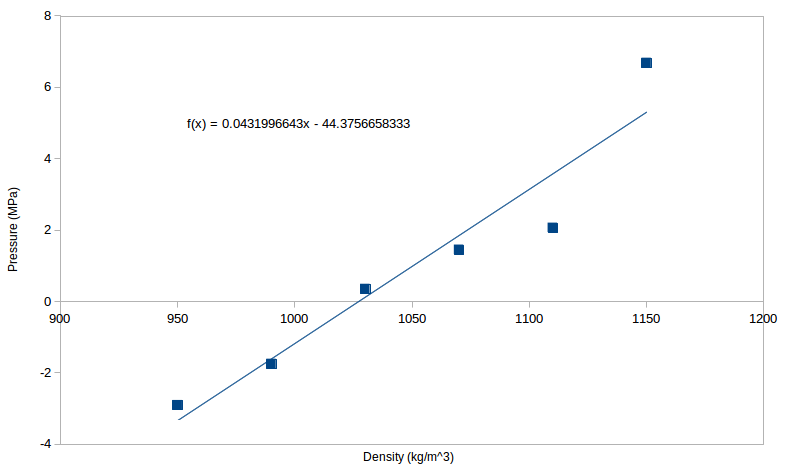
\includegraphics[width=.9\linewidth]{./P1/zero-pressure-density.png}
\caption{\label{fig:P1b}The figure shows the relation between $\rho(kg/m^3)$ with $\langle P \rangle$ (MPa).}
\end{figure}

It is noted that every data point in Fig.\ref{fig:P1b-pressure} for a pressure at given density is obtained by averaging over 3 independent MC runs. Density at zero pressure is found from solving the linear equation resulting in 1017.215 $kg/m^3$, which is at a cell dimension of 7.538. This is in acceptable agreement with the value of 1031 $kg/m^3$ obtained in HM\#4. Better results could be obtained by running the simulation over longer moves and also averaging the data over multiple independent runs.

\section{Problem 2}
\label{sec-2}
\begin{figure}[htb]
\centering
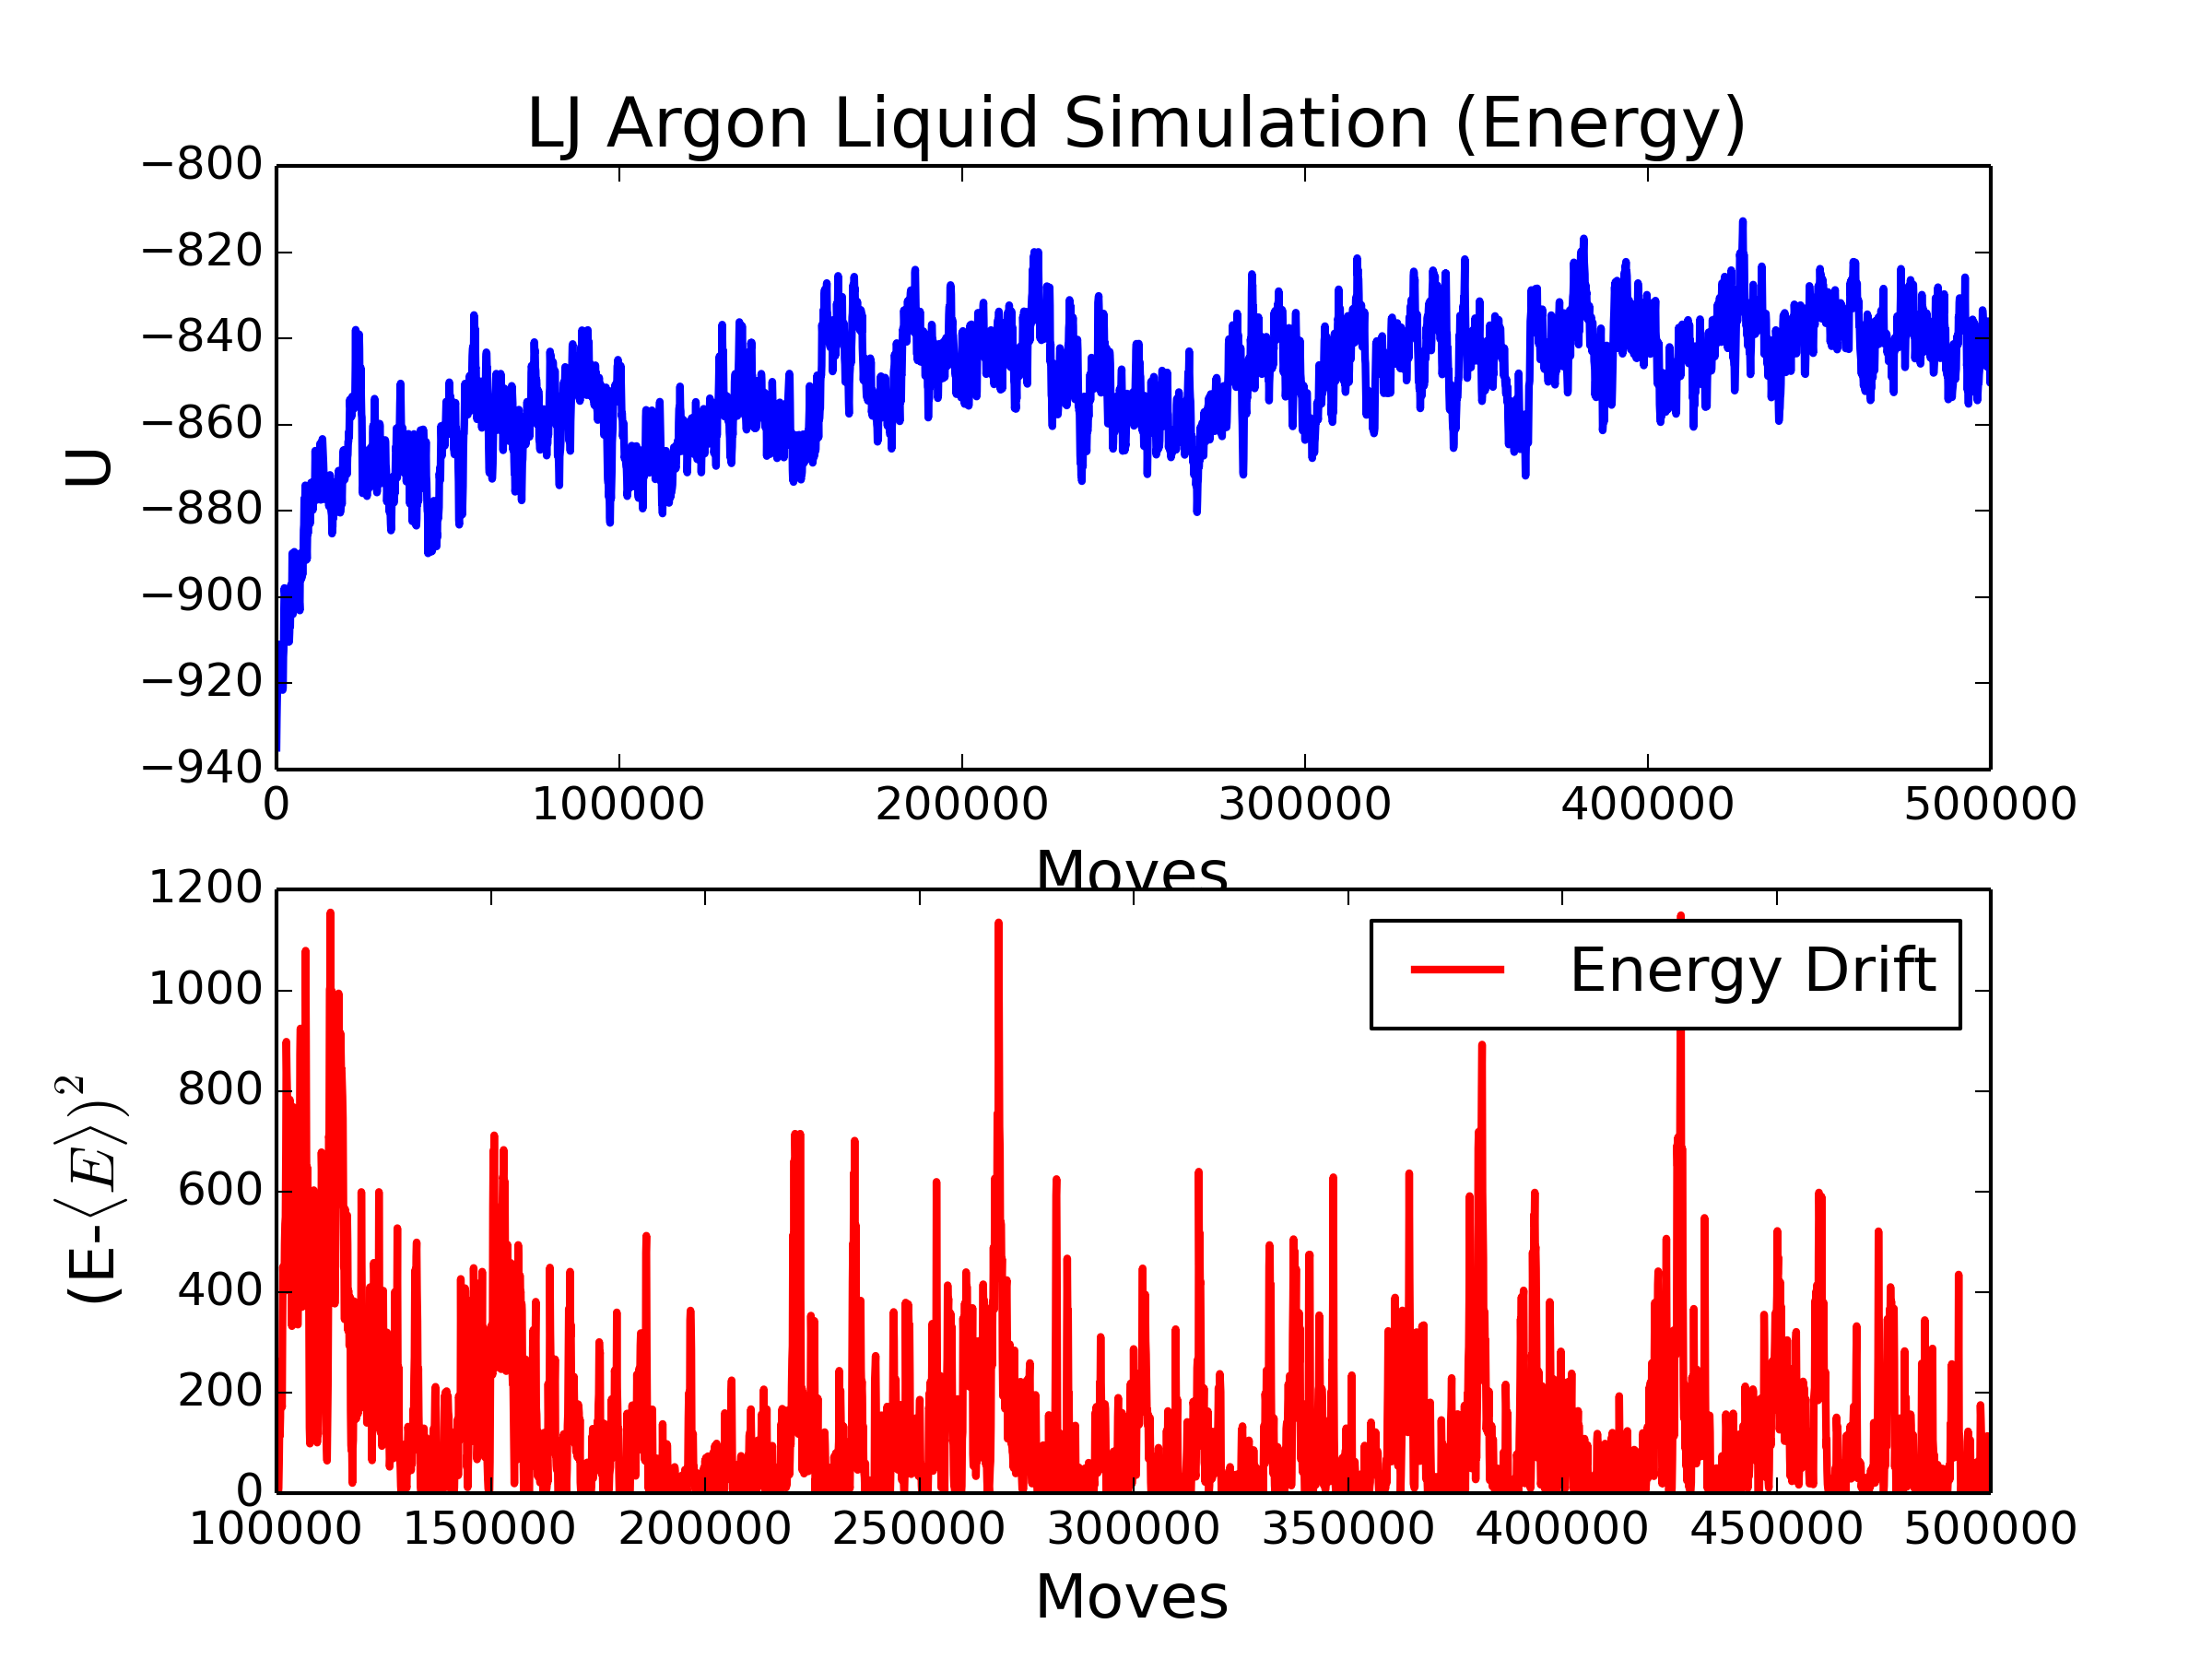
\includegraphics[width=.9\linewidth]{./P2/LJ-md-Ener.png}
\caption{\label{fig:P2}The figure shows the relation between $\rho(kg/m^3)$ with $\langle P \rangle$ (MPa).}
\end{figure}

Metropolis montecarlo simulation is performed at the cell lenth obtained from the zero pressure liquid density. For a good statistical average, the simulation is ran for 500,000 trail moves and, the averaging is performed for the last 400,000 moves. This omits the equilibration period. Total heat capacity is the sum of the following terms, $c_{v,U}$ and $c_{v,K}$. Plot of variation in the potential energy and the drift involved is shown in Fig.\ref{fig:P2}

\begin{equation}
c_{v} = c_{v,U} + c_{v,K}
\end{equation}

Following values are obtained from the simulation, the heat capacity from the potential energy contribution is obtained to be 156.55 J/Kg-K. This is obtained by converting J/K to J/kg-K with the help of mass of one atom (6.63-26 kg).

From the kinetic contribution, 
$$C_{v} = 1.5 k_B$$, which is the heat capacity contribution on per-atom basis
$$C_{v} = 312.3639 J/kg-K}$$, obtained by dividing the above expression with mass of one atom (6.63e-26 kg).

Hence the total heat capcity of the system results to be \textbf{468.9139 J/kg-K} which is in agreement with the value of 460 J/kg-K obtained from the MD simulation.



In terms of computational efficiency, Monte Carlo simuations is recommended though it has issues with the convergence of heat capacity. In terms of fewer computations, MC method would perform far lesser calculations when compared to MD as there is no need for velocity-verlet scheme which determines the positions and in turn depend on the expensive force based calculation. Hence MC is recommended for the determination of heat capacity.
% Emacs 24.5.1 (Org mode 8.2.10)
\end{document}